\documentclass{article}
\usepackage[margin=1in]{geometry}
\usepackage{amsmath}
\usepackage{amssymb}
\usepackage[shortlabels]{enumitem}
\usepackage{xcolor}
\usepackage{pgfplots}
\usepackage{graphicx}
\graphicspath{ {images/} }

\title{\huge \textbf{Theory Assignment 1: Clocks \& Snapshots}}
\author{\Large \textbf{Ganesh Vernekar - CS15BTECH11018}}
\date{}

\begin{document}
  \Large
  \pagenumbering{gobble}
  \maketitle
  \pagenumbering{arabic}

  \renewcommand{\labelenumii}{\Roman{enumii}}
   \begin{enumerate}
   
   \item % Answer 1

   Consider the below timeline. As in Singhal-Kshemkalyanis we send only the changed values, the messages and time at the events are as follows \\~

	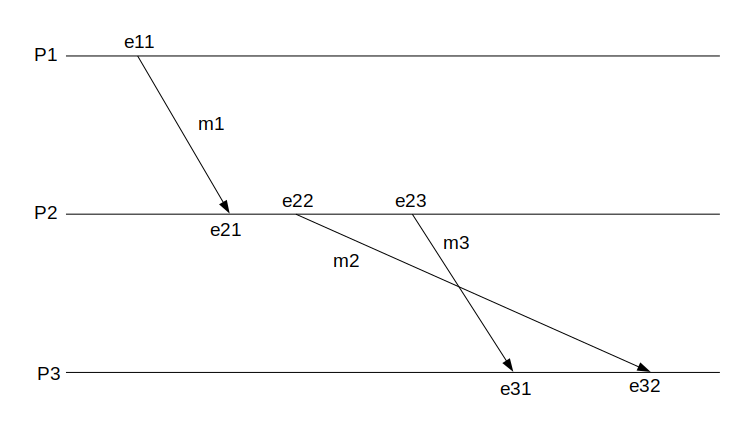
\includegraphics[scale=0.57]{pic1}
	
	(All processes start with clock $[0, 0, 0]$ and increment for every event.)
	
	\begin{minipage}{0.45\textwidth}
	\begin{center}$ $
	$C(e_{11}) = [1, 0, 0] $   \\~
    $C(e_{21}) = [1, 1, 0] $   \\~
	$C(e_{22}) = [1, 2, 0] $   \\~
	$C(e_{23}) = [1, 3, 0]$   \\~
	$C(e_{31}) = [0, 3, 1] $   \\~
	$C(e_{32}) = [1, 3, 2]$   \\~ \\~
	\end{center}
	\end{minipage}
	\hfill
	\begin{minipage}{0.45\textwidth} 
	$m_1 = \{(1,1)\}$ \\~
    $m_2 = \{(1,1), (2,2)\}$ \\~ 
	$m_3 = \{(2,3)\}$ \\~ 
	\end{minipage}%
\\~\\~\\~\\~
	Here $m_2$ and $m_3$ are not FIFO. \\~
	
	From $m_3$, $e_{23} < e_{31}$ \\~
	And $e_{22} < e_{23}$ \\~
	$\therefore e_{22} < e_{31} \implies C(e_{22}) < C(e_{31}) $ --- (1) \\~
	
	But \\~
	$C(e_{22}) \nless C(e_{31})$, $C(e_{31}) \nless C(e_{22})$ \\~
	$\implies C(e_{22}) \parallel C(e_{31})$ --- (2) \\~
	
	(1) and (2) contradict. Hence Singhal-Kshemkalyanis will not work correctly if the channels are not FIFO.
	 
    \item % Answer 2
	\textbf{Modification:} Send control messages only over a spanning tree of the channels.\\~
	
	\textbf{How it works?}
	
	\begin{enumerate}[i.]
		\item Assumption: Initially all nodes are made know about the topology of the systems and the spanning tree in the system.
		\item When a node receives a marker message
		\begin{enumerate}[label=\alph*.]
			\item Take the snapshot as described in Lai-Yang algorithm.
			\item Send marker messages only to the outgoing channels in the spanning tree.
			\item As in the spanning tree there is only 1 incoming edge for every node, send the snapshot to the collector as soon as we send markers to other nodes.
		\end{enumerate}
	\end{enumerate}
	
	\textbf{How O(N)?}
	
	\begin{enumerate}[i.]
	\item The number of marker messages sent are equal to the number of edges in the spanning tree, which is $N-1$ (where $N$ is the number of nodes). Which is $O(N)$.
	
	\item Every node sends its snapshot to the collector, which is again only $N$ messages (1 per node). Which is $O(N)$ again.	
	\end{enumerate}
	
	$\therefore O(N)+O(N) = O(N)$
	
	    
    
   \end{enumerate}
\end{document}